\section{Arquitectura}
\subsection{Conectores propios}
\subsubsection{Notaci'on}

\begin{itemize}
\item Pipe 
\includegraphics[height=0.6cm]{diagramas/NPIPE} 
\item HC (Holy Connector) 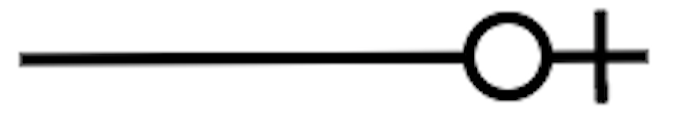
\includegraphics[height=0.5cm]{diagramas/NHC} 
\item AHC (Asynchronous Holy Connector) 
\includegraphics[height=0.5cm]{diagramas/NHCCA}
\item HVC (Holy Video Connector) 
\includegraphics[height=0.5cm]{diagramas/NHVC} 
\item HDC (Holy Data Connector) 
\includegraphics[height=0.5cm]{diagramas/NHDC} 

\end{itemize}

\subsubsection{HC (Holy Connector)}

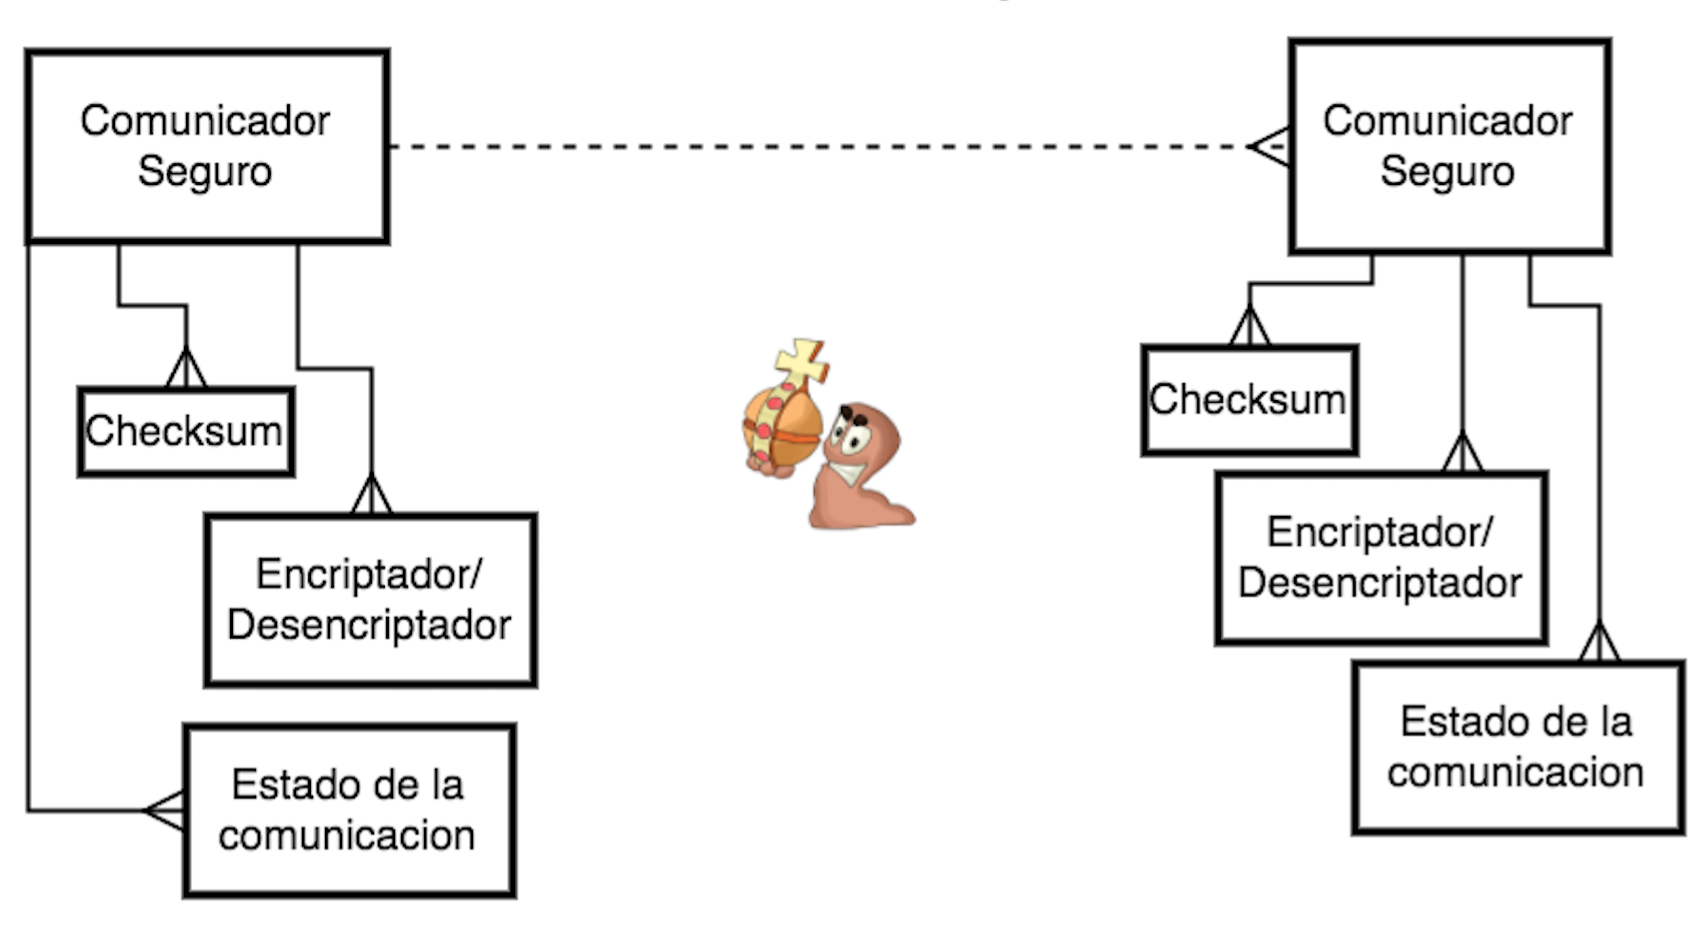
\includegraphics[height=9cm]{diagramas/HC} 

Este conector provee:

\begin{itemize}
	\item \textbf{Seguridad.} Mediante un componente de encriptaci'on y desencriptaci'on de los datos enviados.
	\item \textbf{Integridad.} Mediante un componente de checksum.
	\item \textbf{Confiabilidad de la conexi'on.} Mediante un componente que mantiene el estado de la conexi'on. Por ejemplo, este componente podr'ia implementar el protocolo TCP.
\end{itemize}

Observemos que entre los extremos utilizamos un conector tipo client-server que, asumimos, que se extiende sobre un medio inseguro. Por lo tanto, podemos pensar al Holy Connector como un cliente-server seguro, sobre un medio inseguro.

\subsubsection{AHC (Asynchronous Holy Connector)}

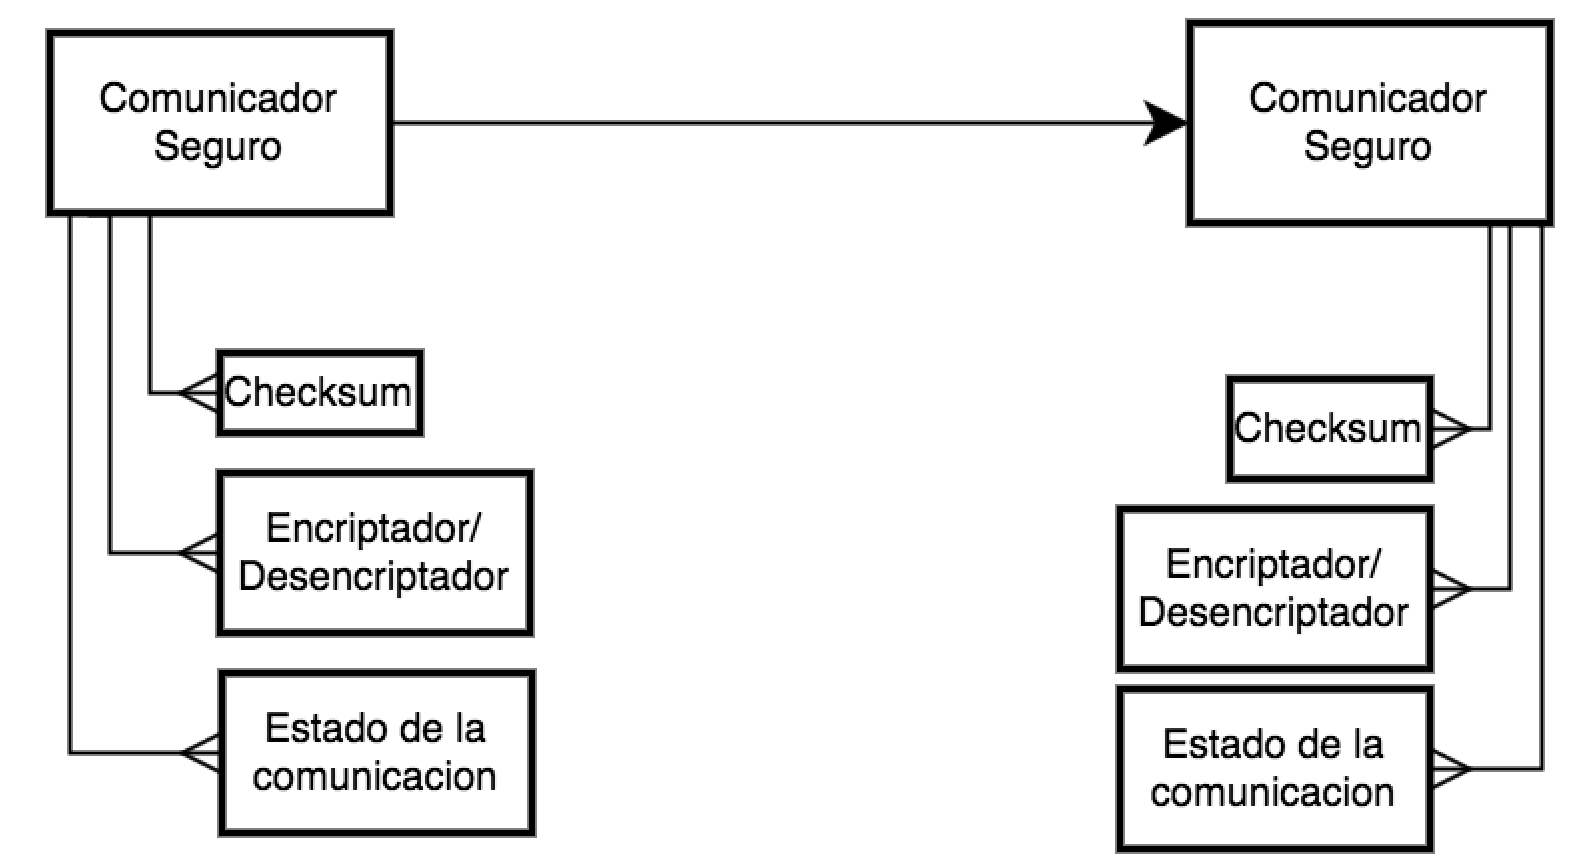
\includegraphics[height=9cm]{diagramas/HCCA} 

Id'entico al Holy Connector, con la diferencia de que en lugar de usar un client-server como conector intermedio, utilizamos un conector de call asincr'onico.

\subsubsection{HVC (Holy Video Connector)}

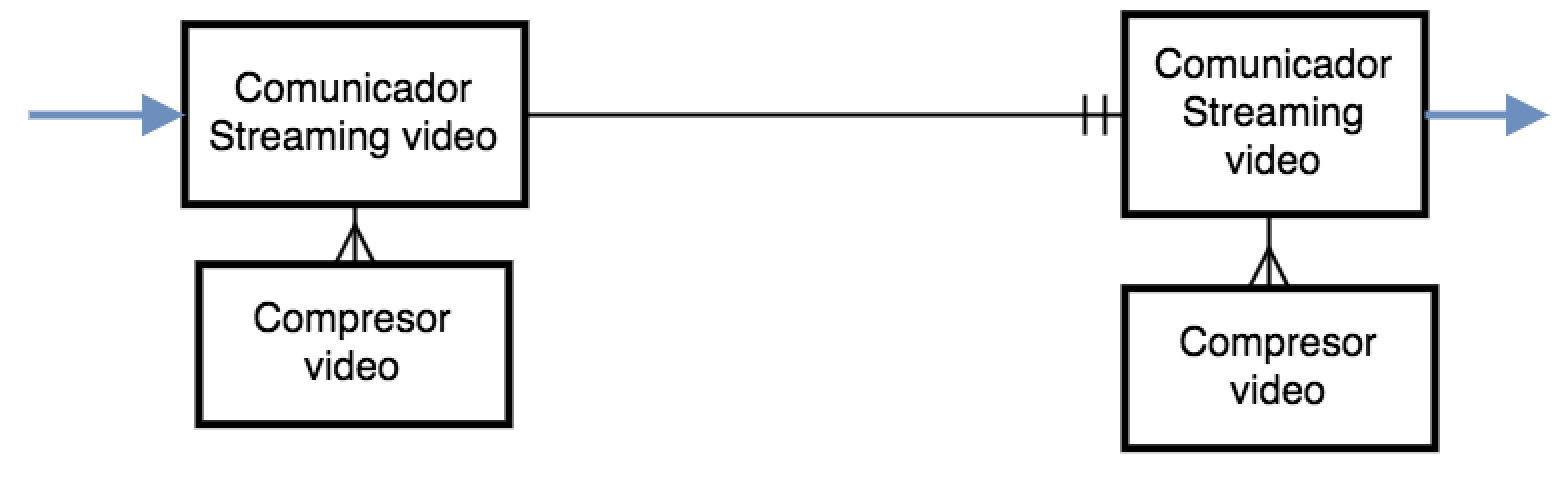
\includegraphics[height=5cm]{diagramas/HVC} 

Contamos en ambos extremos con comunicadores de streaming, que se comunican mediante un Holy Connector. Adicionalmente tenemos, en ambos extremos, compresores adecuados, para que la tasa de cantidad de informaci'on transmitida sea m'as alta.

En ambos extremos tenemos, adem'as, pipes como conectores de entrada y salida. Este buffering permite el env'io y recepci'on de datos flu'ida (evita los tipicos mensajes ``\textbf{buffering...}'').


\subsubsection{HDC (Holy Data Connector)}

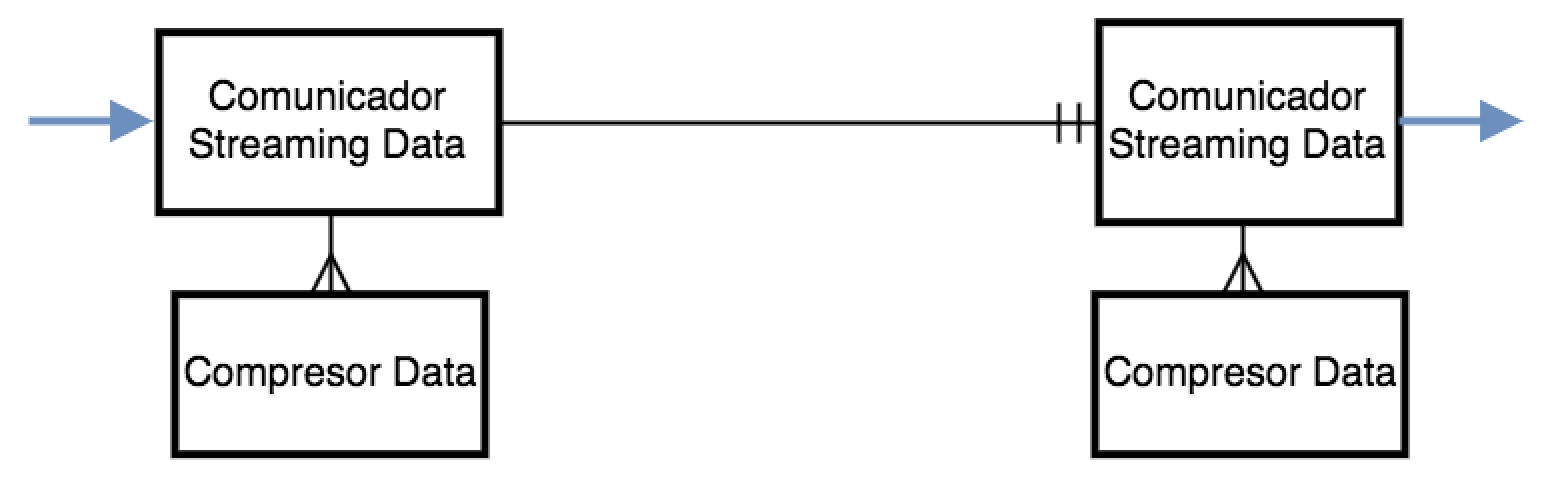
\includegraphics[height=5cm]{diagramas/HDC} 

An'alogo al HVC, pero con compresores adecuados para texto en lugar de video. 

\subsection{Diagrama}

\subsubsection{Arquitectura orientada a datacenters}

Nuestro sistema tiene una arquitectura distribuida, basada en datacenters. Un datacenter contiene una gran cantidad de servidores que proveen el servicio de juego. Dentro de un datacenter, los servidores se dividen en conjuntos, y cada conjunto provee servicio a una regi'on distinta. En otras palabras, un datacenter puede proveer servicio a distintas regiones por medio de cierto conjunto de servidores.

Todas las peticiones ingresantes en un datacenter son recibidas y procesadas por una m'aquina de tipo \textit{router}. Un router redirige la petici'on a alg'un servidor de la regi'on correspondiente. Los routers pueden rutear al conjunto de servidores de cualquiera de las regiones servidas en el datacenter. Por ejemplo, podr'ia haber un datacenter en Argentina, que provea el servicio para Argentina, Brasil y Uruguay; en este caso, los routers del datacenter procesan peticiones de las tres regiones.

El siguiente diagrama muestra lo descripto. 

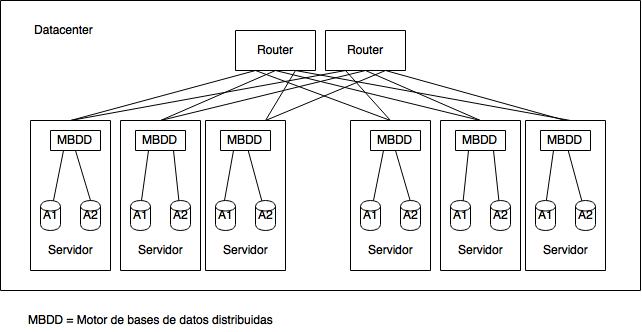
\includegraphics[width=15cm]{diagramas/datacenter.png}

\noindent
El datacenter de la figura tiene dos routers, que procesan pedidos para dos regiones. Cada regi'on se compone de tres servidores. Notar que una de las regiones contiene dos tipos de repositorios, A1 y A2. Estos repositorios aparecen en todos los servidores de la regi'on, debido a que los datos est'an distribuidos sobre todos estos servidores. An'alogamente, los servidores de la otra regi'on, tienen repositorios B1 y B2, distribuidos.

Cada servidor tiene un componente que administra el acceso a los repositorios distribu'idos, que forman parte del sistema de distribuci'on de datos sobre el conjunto de servidores de una regi'on en un datacenter.

Este esquema de distribuci'on de datos sobre servidores es lo que permite que el sistema sea escalable. Adem'as provee otras bondades como capacidad de replicaci'on de datos, necesario para tener alta disponibilidad. M'as a'un, es posible implementar distribuci'on de datos entre datacenters, haciendo que el conjunto de servidores est'e distribu'ido en m'as de un datacenter. Esto se muestra en la siguiente figura.

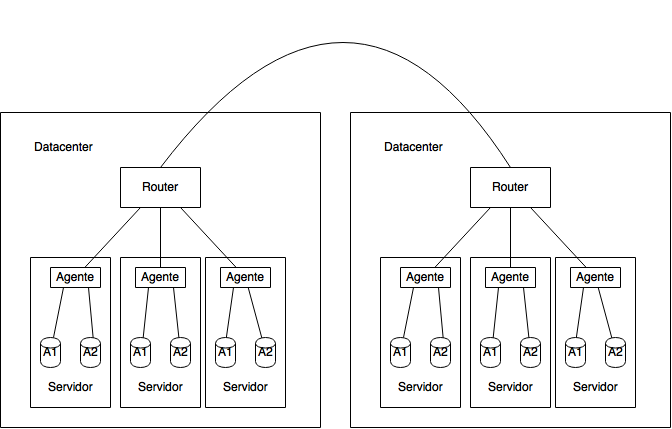
\includegraphics[width=15cm]{diagramas/datacenterx2.png}

\noindent
De esta forma podemos implementar replicaci'on de datos entre datacenters, y as'i si un datacenter se cae, no perdemos datos ni capacidad de proveer servicio a una regi'on.

\subsection{Repositorios distribuidos}

Como dijimos, los repositorios forman parte de un esquema de almacenamiento de datos distribu'ido. Un repositorio distribu'ido en un datacenter contiene, exclusivamente, informaci'on sobre la regi'on que cubre un conjunto de servidores.

\begin{itemize}
	\item \textbf{Apuestas por partido.} Contiene las apuestas involucradas en cada partido en ejecuci'on.
	\item \textbf{Partidos pendientes y en ejecucion.} Contiene los partidos (tanto de desaf'io simulaci'on como fantas'ia) que est'an pendientes y en ejecuci'on.
	\item \textbf{Servidores simulando o transmitiendo partido.} Contiene los servidores que est'an simulando o transmitiendo cada partido.
	\item \textbf{Estad'isticas de jugador.} Contiene informaci'on estad'istica, como por ejemplo la cantidad de partidos ganados y perdidos, de cada jugador.
	\item \textbf{Informaci'on de eventos reales.} Contiene toda la informaci'on sobre eventos reales en los que se basan partidos fantas'ia.
	\item \textbf{Usuarios conectados a desaf'io.} Contiene ID e IP de los usuarios actualmente conectados a la sala de un desaf'io.
	\item \textbf{Regiones habilitadas para jugar.} Contiene las regiones a las que se les puede prestar servicio.
	\item \textbf{Regiones habilitadas para transmisi'on de partidos fantas'ia.} Contiene las regiones a las que se les puede transmitir un partido real desde 'esta regi'on.
	\item \textbf{Datos de jugador.} Contiene los datos de un jugador de la regi'on.
	\item \textbf{Estado de partido en ejecuci'on.} Contiene los datos de estado, por ejemplo puntaje de cada equipo, de los partidos que se est'an ejecutando en este momento.
	\item \textbf{Fixtures de desaf'ios.} Contiene los fixtures actualizados de los desaf'ios que a'un no acabaron. En particular, contiene los fixtures de los desaf'ios que a'un no han empezado.
	\item \textbf{Puntaje por acciones.} Contiene informaci'on sobre los par'ametros que se utilizan para puntuar las acciones que ocurren en un partido fantas'ia.
	\item \textbf{Premios por desaf'io.} Contiene los premios (monetarios y no monetarios) que se otorgan a los participantes desaf'ios que a'un no han acabado.
	\item \textbf{M'etodos de pago.} Contiene la informaci'on sobre los servicios de pago que se aceptan en 'esta regi'on.
	\item \textbf{Informaci'on de redes sociales.} Contiene la informaci'on m'as reciente descargada de redes sociales.
	\item \textbf{Publicidades.} Contiene las publicidades m'as recientes recibidas desde los proveedores de publicidad.
\end{itemize}

\subsubsection{Descripci'on general}

Para describir la arquitectura, optamos por explicar c'omo se satisface cada una de los requerimientos indicados en el enunciado. Para 'esto, decidimos citar textualmente, cada p'arrafo del enunciado, y describir los aspectos del sistema relacionados. Si bien la descripci'on no abarca todos los aspectos del sistema (una explicaci'on exhaustiva demandar'ia demasiado tiempo y espacio), es un buen punto de partida para entender el funcionamiento general del mismo.

\textit{Lo primero que se pretende es que abarque varios de los deportes colectivos más populares del planeta. Además del ya citado básquet, deberá incorporar a las ligas de fútbol, hockey, rugby, béisbol y fútbol americano que se determine tengan mayor número de seguidores (ej. el fútbol español o la NFL estadounidense), y que se consigan empresas que provean datos en tiempo real de la evolución del partido (tanto del desempeño de los jugadores como del partido en general). Esto último es importante porque además de la simulación de los mismos, ahora también se quiere incorporar un modo de liga de fantasía tradicional.}

Para agregar deportes, lo 'unico que se debe hacer es contratar nuevos servicios de transmisi'on de partidos, agregar nuevos par'ametros del juego (i. e. agregar datos al repositorio de \textit{puntajes por acci'on}), y agregar funcionalidad al \textit{administrador de desaf'ios} para que se puedan crear desaf'ios de 'este nuevo deporte.

Los datos de la evoluci'on del partido provienen de los mismos servicios que nos transmiten partidos reales. Tanto los datos de un partido, como la transmisi'on del mismo nos son transmitidos en conjunto. Ver componente \textit{Servicio de transmisi'on de partido real}.

\textit{En este nuevo modo los ganadores de los desafíos ya no se deciden a través de la simulación directa de los partidos, sino del desempeño de los jugadores en partidos reales en las ligas en cuestión. Por ej. usando el caso del básquet, se podría otorgar 1 punto por cada punto que haga ese jugador en el partido, 1.5 puntos por cada asistencia, 2 por cada bloqueo o robo, -1 por cada pérdida de balón, etc... El equipo que tenga mayor suma, gana el desafío.}

El puntaje que se asigna a cada acci'on de cada deporte es un par'ametro que se encuentra en el repositorio \textit{puntajes por acci'on}.

\textit{Con respecto a los desafíos, ahora pueden incluir un gran número de partidos, no sólo uno. En el caso de este nuevo modo ``liga fantasía tradicional'', podrían incluirse todos los partidos de una fecha determinada de una liga, o un salteado de un conjunto de fechas cualesquiera, o incluso la liga o torneo completo.
En el caso de la simulación, se arman torneos de diferentes formatos (se elige al momento de plantearse el desafío, playoff, liga, combinado zonas, etc.) con todos los equipos participantes. En este último caso se agrega la duración total “artificial” del torneo en semanas, pues se pretende que los partidos no se resuelvan más de forma inmediata si no que puedan “vivirse” como los
reales (más información luego).
}

Los desaf'ios son creados por un cliente (un jugador o un administrador) desde la pantalla de lista de desaf'ios, mediante el m'odulo \textit{creador de desaf'ios}. 'Este se comunica con un \textit{administrador de desaf'ios}, del lado del servidor, el cual, mediante el \textit{administrador de fixtures}, crea el fixture correspondiente al desaf'io. El fixture puede tener diversas formas, dependiendo del tipo de desaf'io creado, por ejemeplo una liga, un torneo o un partido individual. El fixture es escrito en el repositorio \textit{fixtures de desaf'ios}.

Para que los desaf'ios se puedan extender a lo largo del tiempo, y se puedan vivir como si fuesen reales, existe la posibilidad de que los partidos de un desaf'io comiencen en distintos momentos. Esta informaci'on se incluye en el fixture.

Como los partidos comienzan en distintos momentos, el sistema contiene un m'odulo \textit{dispatcher de partidos simulaci'on} que sensa regularmente los fixtures, buscando los pr'oximos partidos a ejecutarse. Cuando llega la hora de ejecutar un partido, le informa al \textit{simulador de partido} que debe comenzar a ejecutar una simulaci'on. Le transmite la informaci'on de los equipos y los datos de los usuarios involucrados. Cuando el simulador concluye la ejecuci'on, le informa el resultado al \textit{procesador de resultados}.

Por un lado, este m'odulo le comunica al \textit{administrador de pagos} el ganador y el perdedor del partido, para que 'este efect'ue el pago correspondiente, seg'un las apuestas. Las apuestas se encuentran en el repositorio \textit{apuestas por partido en ejecuci'on}. Con toda esta informaci'on, el administrador de pagos le indica al sistema de pagos externo, las transacciones a realizarse.

Por otro lado, al terminar la simulaci'on, se le informa al administrador de fixtures c'omo debe modificar el fixture. Otros repositorios tambi'en son modificados adecuadamente.

\textit{No sólo los jugadores pueden crear desafíos, sino que administradores propios del sitio pueden crearlos. Queda claro, que ahora los desafíos pueden ser aceptados por miles de jugadores, que competirán cada uno con su equipo para salir vencedor.}

Los desaf'ios pueden ser creados desde un programa cliente hecho espec'ificamente para administradores.

\textit{
Cada desafío tendrá un chat general para intercambiar mensajes con otros participantes, además de las conversaciones que podrá tener con competidores amigos a modo de ``Instant Messenger'' a través de la plataforma.
}

Se incluye la posibilidad de chatear en las pantallas de partido. Un \textit{receptor/enviador de mensajes de chat} se encarga de recibir mensajes de chat, distribuirlos a todos los usuarios conectados a una sala, y filtrar y analizar aquellos que se refieran a jugadores de alguno de los equipos del partido, para modificar sus estad'isticas en tiempo real. Las modificaciones de las estad'isticas de los deportistas son almacenadas en el repositorio \textit{estad'isticas de deportistas}.

\textit{
La idea principal con mayor consenso en los inversores, es que las fichas de apuesta pasan a ser reemplazadas por dinero real. Todos los participantes deberán poder ingresar datos de una tarjeta de crédito o cuenta corriente en entidades bancarias de los países participantes para que el sistema pueda debitar o acreditar dinero de forma inmediata y ser registrados por el sistema de forma segura.
}

Justo antes de comenzar un partido, ocurre una ronda de apuestas entre los jugadores involucrados. Las apuestas, solicitadas por un \textit{administrador de apuestas}, se crean en el cliente por medio de un \textit{creador de apuestas}. Recibidas las apuestas en el servidor, el administrador las almacena en el repositorio \textit{apuestas por partido en ejecuci'on}.

\textit{
Si bien el juego sigue permitiendo jugar absolutamente gratis, existirán desafíos que tengan una cuota de entrada para participar y repartirán un monto de dinero en premios en base a una cantidad mínima de participantes que deben anotarse para que el mismo pueda realizarse. Los premios que se pagarán serán en relación al rango de posiciones en el que queda el equipo del jugador al terminar el desafío (ej: 1er puesto, 2do, 3ro, 4to a 10mo, 10 a 50, 50 a 200, 200 a 1000, etc.).
Los desafíos “gratis” pueden otorgar premios como créditos no retirables para jugar, productos exclusivos de “partners”, tickets para eventos deportivos, etc.
}

La cuota de entrada y los premios no monetarios se fijan a la hora de crear un desaf'io, y son procesados por el administrador de desaf'ios. Esta informaci'on es almacenada en el repositorio \textit{premios por desaf'io}.

\textit{Una vez que comienza el primer partido de un desafío ya no se pueden hacer cambios en el equipo registrado o salirse del mismo o ingresar nuevos participantes. Cada desafío deberá tener una cuenta regresiva para indicar el tiempo restante para el comienzo. En todo momento, incluso mientras los partidos se están desarrollando, se debe poder ver quiénes son los participantes del mismo y el puesto actual del equipo del participante en el desafío actualizado al minuto a minuto de los partidos.}

Para inscribirse a un desaf'io, un usuario utiliza el \textit{listador de desaf'ios} que, adem'as de mostrar todos los desaf'ios disponibles, permite inscribirse a ellos. La informaci'on de la inscripci'on es enviada a un administrador de desaf'ios, que le ordena al administrador de fixtures modificar el fixture con el nuevo inscripto. Comenzado un desaf'io, el administrador de fixtures no aceptar'a ning'un cambio sobre el fixture. Por lo tanto, no habr'a nuevas inscripciones.

Asimismo es posible recuperar la informaci'on sobre los participantes de un desaf'io en curso, a trav'es del fixture del desaf'io. Los rankings de un desaf'io son confeccionados por un \textit{calculador de rankings} que, bas'andose en un fixture, calculan la posici'on de cada jugador.

\textit{
De hecho, el estado de los partidos de los desafíos (en cualquiera de sus modos) debería poder seguirse en vivo a través del sitio, como cualquier sitio de noticias deportivo. Además, se está muy avanzado en conversaciones para acceder a streams de videos de diferentes ligas y que el partido pueda seguirse legalmente a través de la plataforma en algunas regiones habilitadas. Los dueños de los derechos de transmisión, a cambio, quieren poder vender espacios de publicidad en el sitio y acceder a algunos datos de preferencias/comportamiento de los usuarios, además de sus cuentas de mails para efectuar campañas de marketing más específicas.
}

Cuando un usuario ingresa a la sala de un desaf'io, se conecta a un servidor que est'e simulando o proveyendo una transmisi'on de partido real, y 'este comienza a transmitirle datos.

En el caso del modo fantas'ia, el permiso de acceso a una transmisi'on est'a almacenado en el repositorio \textit{regiones habilitadas para transmisi'on de partidos fantas'ia}. Cuando un usuario solicita acceso a la sala de un desaf'io, primero debe resolverse la ubicaci'on de un datacenter que contenga la informaci'on sobre ese desaf'io. Ubicado un tal datacenter, se verifica el permiso de acceso a la transmisi'on, y en caso que la regi'on del usuario est'e habilitada, se le concede acceso a un servidor que est'e proveyendo la transmisi'on.

A los due\~nos de los derechos de transmisi'on se les puede dar acceso a los repositorios de datos de usuarios f'acilmente, consultando cualquiera de los datacenters. A su vez, tenemos almacenadas publicidades que ser'an mostradas en pantallas de desaf'ios. Las publicidades son recibidas a trav'es de proveedores de publicidad externos, y almacenadas en un repositorio \textit{publicidades}.

\textit{
Con respecto al modo de simulación, se pretende extender las reglas utilizando a un comité de expertos (jugadores, técnicos, estadísticos, periodistas deportivos, etc.) de cada deporte para intentar que se asemeje aún más a la realidad. En el caso del básquet incorporará fouls, tiros libres, cambios de jugadores (suplentes), minutos en cancha + cansancio, tiempos con cambios de lado de la cancha, estadios locales y visitantes, condiciones climáticas, movimiento de los jugadores y sus posiciones en la cancha al efectuar acciones, etc. para extrapolar más certeramente la actuación del jugador en base a sus estadísticas.

Al mismo tiempo se busca modificar el simulador para que en vez de un log de salida, provea un stream continuo de “minuto a minuto” mucho más detallado que el log de la versión anterior. La razón de esta decisión es que se está por llegar a un acuerdo por la compra de un motor gráfico que permita a los participantes ver el partido a partir del stream de salida del simulador. En este momento se negocia por al menos dos motores diferentes.
}

Las reglas de los juegos simulados est'an completamente contenidas en el simulador. Su modificaci'on no afecta al funcionamiento del resto de nuestro sistema.

Un simulador de partido, ubicado en el servidor, env'ia un flujo de datos a todos los clientes conectados al mismo. Cuando un cliente recibe datos de la simulaci'on, son procesados por un motor gr'afico, el cual posteriormente los dibuja en la interfaz gr'afica.

\textit{
El primero es un motor gráfico 3d de última generación que muestra a los jugadores con un gran nivel de realismo pero que puede ser muy pesado para la mayoría de los dispositivos con los que los participantes accederían al portal (que va desde PCs de escritorio a dispositivos móviles de todo tipo). La empresa desarrolladora habla de que se le podría diseñar un módulo para transmitir en video el partido a los dispositivos no soportados por el motor gráfico. Otra empresa presenta un motor 2d más humilde pero mucho menos demandante, donde los partidos se ven “desde arriba” con un diseño caricaturezco y que funciona para dispositivos móviles con varios años de antigu\"uedad. Se cree que se va a llegar a un acuerdo con ambas compañías para incorporar ambos motores en la primera versión, según se necesite.
}

Se decidi'o incluir ambos motores gr'aficos en el programa cliente. Por lo tanto, cuando se detecte que el dispositivo cliente no tiene prestaciones suficientemente buenas para utilizar el motor 3D, se utilizar'a el motor 2D. No se enviar'an datos de video 3D preprocesados desde el servidor.

\textit{
Cualquier participante, incluso si no forma parte del desafío debería poder ver un partido simulado de su región. Al ser ahora “visibles” las simulaciones, las mismas dejan de ser instantáneas, y se intenta que las duraciones sean similares a las de un partido normal. De esta forma se puede vender publicidad específica a través del sitio. También se quiere aumentar el caudal de redes sociales que se utilizan para “afectar” las estadísticas (no sólo Twitter, sino incorporar Facebook, Google+, etc.) y que incluso los comentarios de los usuarios en los chats de los desafíos o incluso los IMs (Instant Messages) privados de los usuarios puedan ser utilizados para afectar los resultados. Como las simulaciones ahora duran similarmente a un partido real, los resultados de menciones pueden verse como un “rating minuto a minuto” de cada jugador.
}

Un usuario puede solicitar ver cualquier partido de la lista de desaf'ios y, si su regi'on est'a habilitada, un servidor adecuado se lo transmitir'a. La duraci'on del partido estar'a dado por el flujo de datos transmitido del servidor al cliente.

Las redes sociales son constantemente sensadas por un \textit{administrador de redes sociales}, que se encarga de extraer datos relevantes relacionados con deportes. Estos datos son almacenados en un repositorio \textit{informaci'on de redes sociales}. Esta informaci'on es sensada peri'odicamente por un \textit{analizador de informaci'on de redes sociales}, el cual procesa la informaci'on y se la transmite al simulador de partido. Adem'as, actualiza el repositorio de estad'isticas de jugadores.

\textit{Se espera que el sistema sea utilizado por millones de personas a lo largo y ancho del planeta y que se llegue a ese número de suscriptos muy rápidamente (hay mucho interés de que uno de los países incluidos en la versión inicial sea China). Algunos especialistas en redes plantearon entonces la necesidad de regionalizar la plataforma en varios niveles y que los participantes de cada región sólo compitan entre sí en desafíos locales o nacionales (que puede ser de las ligas del mundo más seguidas para esa región). Además, se cree, esto debería facilitar la logística con los bancos, el idioma de los chats, los pagos en la moneda local, la entrega de premios, etc.
}



\subsubsection{Atributos de Calidad vs Arquitectura}
A continuacion listamos todos los atributos de calidad detallados en la seccion anterior y explicamos como hicimos para resolverlo en el diagrama de componentes y conectores.

\begin{itemize}
\item Atributo: El sistema debe evitar que los servidores superen su l'imite de clientes y se caigan.
\item Justificaci'on: Los componentes \textit{router} que reciben las peticiones de un cliente mantienen contadores acerca de la carga de los servidores. Cuando detectan una posible sobrecarga consultan la cantidad de usuarios conectados a los servidores de una regi'on. Lo hacen consultando el repositorio \textit{usuarios conectados a desaf'io}. Si hay sobrecarga, no se responde a las peticiones.

\item Atributo: Desea que haya un esfuerzo por respetar a los países en los que su legislación no permite que directamente se ingrese al sitio.
\item Justificacion: Los \textit{router} que reciban peticiones provenientes de regiones no habilitadas, no ser'an resueltas. Las regiones no habilitadas se consultan en el repositorio \textit{regiones habilitadas para jugar}.

\item Atributo: Se requiere que sea fácil desactivar una cuenta por un tiempo, para ayudar a los adictos en recuperación.
\item Justificacion: Se incluye un m'odulo para desactivar una cuenta, en el programa cliente.

\item Atributo: El simulador debe poder extenderse para soportar reglamentaciones nuevas ya que se espera poder incluir pa'ises adicionales.
\item Justificacion: La modificabilidad el simulador corre por cuenta de los desarolladores del mismo. En el caso del modo fantas'ia, cuya operatoria depende de nuestros desarrolladores, se incluye un repositorio con datos de configuraci'on para los partidos de dicho modo.

\item Atributo: El sistema debe correr en la mayor cantidad de plataformas posible. El sistema debe poder extenderse f'acilmente para incluir nuevas plataformas.
\item Justificacion: La arquitectura del sistema no asume requerimientos de hardware o software (salvo algunos muy b'asicos) sobre el cliente. Para poder soportar todo el abanico de dispositivos, desde aquellos con recursos de hardware y software limitados como aquellos de altas prestaciones, se incluyen dos motores gr'aficos, uno 3D (de altos requerimientos) y otro 2D (de bajos requerimientos). La decisi'on sobre cu'al utilizar se toma en base a los recursos disponibles al momento de la recepci'on de los resultados de la simulaci'on.

\item Atributo: 
\item Justificacion:

\item Atributo: 
\item Justificacion:

\item Atributo: 
\item Justificacion:
\end{itemize}

